\documentclass[12pt,a4paper]{article}
% компилировать xelatex: xelatex report.tex (дважды)
\usepackage{fontspec}
\setmainfont{FreeSerif}
\setsansfont{FreeSans}
\setmonofont{DejaVu Sans Mono}[Scale=0.85]
\usepackage{polyglossia}
\setdefaultlanguage{russian}
\usepackage{amsmath,amssymb}
\usepackage{graphicx}
\usepackage{booktabs}
\usepackage{float}
\usepackage[margin=2cm]{geometry}
\usepackage{listings}
\usepackage{xcolor}
\usepackage[hidelinks]{hyperref}
\makeatletter\newcommand\inputtable[1]{\@@input #1 }\makeatother
\lstset{basicstyle=\ttfamily\small,columns=fullflexible,frame=single,breaklines=true}
\newcommand{\eps}{\varepsilon}

\begin{document}

\begin{titlepage}
\centering
{\large Московский государственный университет имени М.\,В.~Ломоносова\\
Факультет вычислительной математики и кибернетики\par}
\vspace{5cm}
{\Large\bfseries Отчёт по заданию курса\\
<<Суперкомпьютерное моделирование и технологии>>\par}
\vspace{1cm}
{\large Численное решение задачи Дирихле для уравнения Пуассона\\
в криволинейной области методом фиктивных областей\par}
\vspace{1cm}
{\large Вариант 19\par}
\vfill
\begin{flushright}
Выполнил: студент 608 группы\\[1mm]
Джамалдинов Рамзан Русланович
\end{flushright}
\vspace{1cm}
Москва, 2026
\end{titlepage}

\tableofcontents
\newpage

\section{Математическая постановка задачи}

В области $D\subset\mathbb{R}^2$, ограниченной кусочно-гладким контуром $\gamma$,
рассматривается уравнение Пуассона с граничным условием Дирихле
\begin{equation}\label{eq:pois}
-\Delta u = f(x,y),\quad (x,y)\in D,\qquad u(x,y)=\varphi(x,y),\quad (x,y)\in\gamma,
\end{equation}
где $f(x,y)=1$, $\varphi(x,y)=\sin(x+y)$.

\textbf{Вариант 19.} Область $D$~--- часть квадрата $\{-2<x,y<2\}$, лежащая вне окружности
$x^2+(y-2)^2=1$:
\[
D=\{(x,y):\ -2<x<2,\ -2<y<2,\ x^2+(y-2)^2>1\}.
\]
Центр окружности $(0,2)$ лежит на верхней стороне квадрата, поэтому из квадрата
вырезается нижний полукруг радиуса 1. Граница $\gamma$ состоит из трёх сторон квадрата
($x=\pm2$, $y=-2$), двух отрезков верхней стороны $y=2$, $1\le|x|\le2$, и нижней
полуокружности $x^2+(y-2)^2=1$, $y\le2$.

\section{Метод фиктивных областей}

В качестве прямоугольника выбран $\Pi=\{-2<x<2,\ -2<y<2\}$ (то есть $A_1=A_2=-2$,
$B_1=B_2=2$), его граница $\Gamma$. Фиктивная область~--- нижний полукруг
\[
\hat D=\Pi\setminus D=\{(x,y):\ x^2+(y-2)^2\le1,\ y<2\}.
\]
Внешняя часть контура $\gamma$ совпадает с $\Gamma$, поэтому граничное условие на ней
ставится точно. На отрезке $\{|x|<1,\ y=2\}$ границы $\Gamma$, принадлежащем фиктивной области,
используется продолжение $v_0$ функции $\varphi$.

В $\Pi$ решается задача
\begin{equation}\label{eq:fict}
-\Delta v + Q(x,y)\,(v-v_0)=F(x,y),\ (x,y)\in\Pi\setminus\gamma,\qquad v=v_0,\ (x,y)\in\Gamma,
\end{equation}
\[
Q=\begin{cases}0,&(x,y)\in D,\\ 1/\eps^2,&(x,y)\in\hat D,\end{cases}\qquad
F=\begin{cases}f(x,y)=1,&(x,y)\in D,\\ 0,&(x,y)\in\hat D,\end{cases}
\]
с условием непрерывности нормальной компоненты потока на $\gamma$. В качестве продолжения
граничной функции взята $v_0(x,y)=\sin(x+y)$~--- гладкая функция во всём $\Pi$.
Известно, что $\max_D|v-u|<C\eps$. По заданию $\eps=h^2$, $h=\max(h_1,h_2)$.

\section{Разностная схема}

В $\bar\Pi$ вводится равномерная сетка $x_i=A_1+ih_1$, $i=\overline{0,M}$, $y_j=A_2+jh_2$,
$j=\overline{0,N}$, $h_1=4/M$, $h_2=4/N$. Во внутренних узлах
\begin{equation}\label{eq:scheme}
-w_{\bar xx,ij}-w_{\bar yy,ij}+Q_{ij}w_{ij}=F_{ij}+Q_{ij}v_0(x_i,y_j),\quad i=\overline{1,M-1},\ j=\overline{1,N-1},
\end{equation}
на границе $w_{ij}=v_0(x_i,y_j)$, $(x_i,y_j)\in\Gamma$; граничные значения перенесены в правую часть.
Коэффициенты
\[
Q_{ij}=\frac{1}{\eps^2}\Bigl(1-\frac{S_{ij}}{h_1h_2}\Bigr),\qquad
F_{ij}=\frac{S_{ij}}{h_1h_2}\,f(x_i,y_j)=\frac{S_{ij}}{h_1h_2},
\]
где $S_{ij}=\mathrm{mes}(\Pi_{ij}\cap D)$, $\Pi_{ij}=[x_{i-1/2},x_{i+1/2}]\times[y_{j-1/2},y_{j+1/2}]$.
Если $\Pi_{ij}\subset D$, то $F_{ij}=f(x_i,y_j)$, если $\Pi_{ij}\subset\hat D$, то $F_{ij}=0$.
Поскольку $f\equiv1$, выбор точки $(x_i^*,y_j^*)$ не влияет на результат.

\textbf{Вычисление площадей.} В программе площадь $S_{ij}$ вычисляется \emph{точно}
(без замены дуги отрезком). Нижняя полуокружность~--- график $g(x)=2-\sqrt{1-x^2}$, $|x|\le1$.
Для прямоугольника $[x_a,x_b]\times[y_a,y_b]$, $y_b\le2$,
\[
\mathrm{mes}\bigl([x_a,x_b]\times[y_a,y_b]\cap\hat D\bigr)=I(y_b)-I(y_a),\qquad
I(t)=\int_{x_a}^{x_b}\max\bigl(0,\ t-g(x)\bigr)\,dx .
\]
При $t\le1$ $I(t)=0$, иначе подынтегральная функция положительна при $|x|<s=\sqrt{1-(2-t)^2}$ и
\[
I(t)=(t-2)(\beta-\alpha)+P(\beta)-P(\alpha),\quad \alpha=\max(x_a,-s),\ \beta=\min(x_b,s),\quad
P(x)=\tfrac12\bigl(x\sqrt{1-x^2}+\arcsin x\bigr).
\]
Тогда $S_{ij}=h_1h_2-\mathrm{mes}(\Pi_{ij}\cap\hat D)$.

Оператор $A$ схемы самосопряжён и положительно определён в пространстве $H$ сеточных
функций со скалярным произведением $(u,v)=\sum_{i,j}h_1h_2u_{ij}v_{ij}$.

\section{Метод решения СЛАУ}

Система $Aw=B$ решается методом сопряжённых градиентов с диагональным предобуславливателем
$(Dw)_{ij}=(2/h_1^2+2/h_2^2+Q_{ij})\,w_{ij}$. Начальное приближение $w^{(0)}=0$, первая итерация
~--- метод скорейшего спуска:
\[
r^{(0)}=B,\ z^{(0)}=D^{-1}r^{(0)},\ p^{(1)}=z^{(0)},\
\alpha_k=\frac{(z^{(k-1)},r^{(k-1)})}{(Ap^{(k)},p^{(k)})},\ w^{(k)}=w^{(k-1)}+\alpha_kp^{(k)},
\]
\[
r^{(k)}=r^{(k-1)}-\alpha_kAp^{(k)},\ z^{(k)}=D^{-1}r^{(k)},\
\beta_{k+1}=\frac{(z^{(k)},r^{(k)})}{(z^{(k-1)},r^{(k-1)})},\ p^{(k+1)}=z^{(k)}+\beta_{k+1}p^{(k)}.
\]
Критерий остановки: $\|w^{(k+1)}-w^{(k)}\|_E=|\alpha_{k+1}|\,\|p^{(k+1)}\|_E<\delta$, $\delta=10^{-8}$;
дополнительно число итераций ограничено числом неизвестных $(M-1)(N-1)$.
Предобуславливатель особенно важен здесь: в фиктивной области $Q_{ij}=h^{-4}$
и без масштабирования диагонали число обусловленности матрицы было бы огромным.

\section{Последовательная программа и результаты на сгущающихся сетках}

Программа \texttt{seq.cpp} (общая часть~--- \texttt{common.h}). Сеточные функции хранятся
в массивах размера $(M+1)(N+1)$, граничные элементы равны нулю, поэтому оператор $A$
применяется без проверок на границе. Время замерялось для всего расчёта
(формирование коэффициентов и итерации), без записи результата в файл.

\begin{table}[H]\centering
\caption{Последовательная программа, $\delta=10^{-8}$}
\begin{tabular}{cccc}\toprule
$(M,N)$ & $\eps=h^2$ & Число итераций & $\|w^{h}-w^{h/2}\|_C$ \\\midrule
$(20,20)$ & $0.04$ & 66 & $2.36\cdot10^{-2}$ \\
$(40,40)$ & $0.01$ & 130 & $3.56\cdot10^{-2}$ \\
$(80,80)$ & $0.0025$ & 256 & $2.63\cdot10^{-2}$ \\
$(160,160)$ & $6.25\cdot10^{-4}$ & 494 & $1.65\cdot10^{-2}$ \\\bottomrule
\end{tabular}
\end{table}
В последнем столбце~--- максимум разности решений на соседних сетках в общих узлах.
Число итераций растёт примерно пропорционально $\max(M,N)$, как и ожидается для
метода сопряжённых градиентов с диагональным предобуславливанием.

\subsection*{Сходимость итерационного метода}
Для контроля работы метода на каждой итерации вычислялись норма
$\|w^{(k+1)}-w^{(k)}\|_E$ (критерий остановки) и функционал
$J(w^{(k)})=-0.5\,(B+r^{(k)},w^{(k)})$ (запуск \texttt{./seq M N delta - trace.txt}).
Функционал убывает монотонно: нарушения монотонности возникают только на последних
итерациях и имеют относительную величину менее $10^{-14}$, то есть находятся на уровне
ошибок округления. Перезапуск метода не требуется.

\begin{figure}[H]\centering
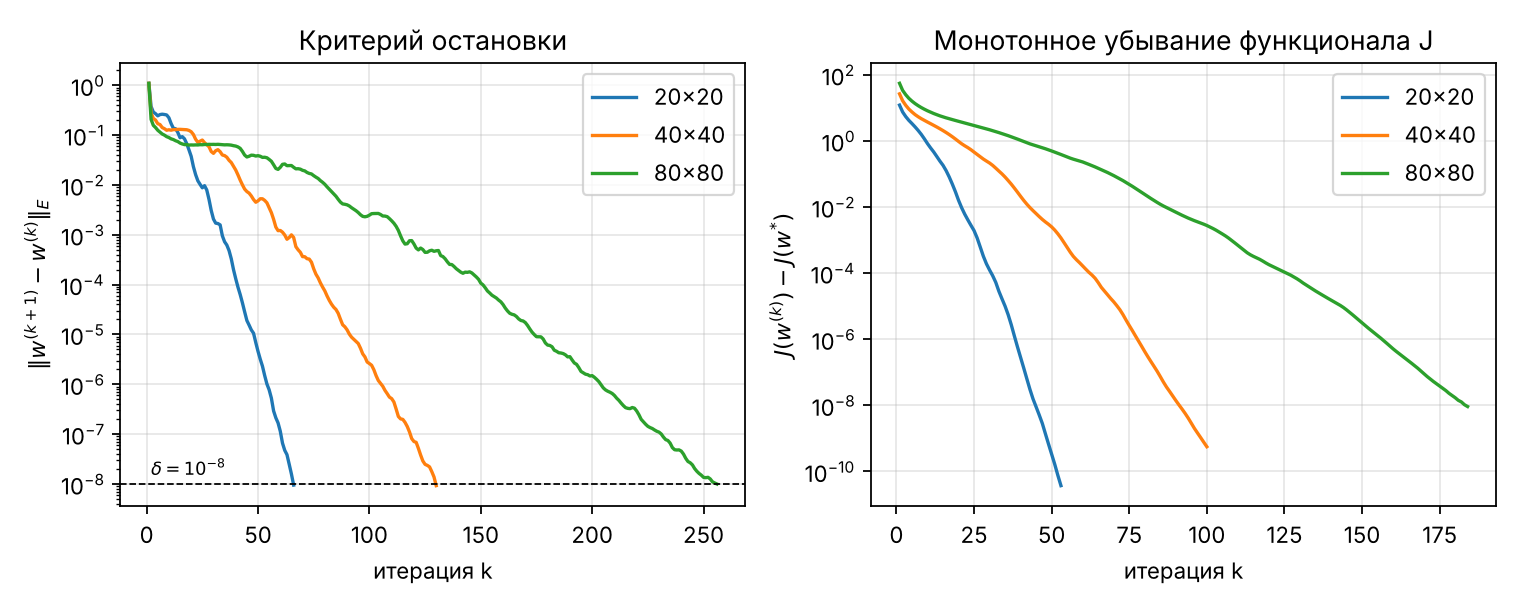
\includegraphics[width=\textwidth]{fig/conv_cg.png}
\caption{Сходимость метода сопряжённых градиентов на сетках $20\times20$, $40\times40$, $80\times80$}
\end{figure}

Поитерационная ошибка оценивалась относительно решения разностной схемы $w^{*}$, полученного
с точностью $\delta=10^{-12}$ (запуск \texttt{./seq M N 1e-8 - trace.txt ref.txt}): на каждой
итерации в журнал записываются $\|w^{(k)}-w^{*}\|_E$ и $\|w^{(k)}-w^{*}\|_C$ по узлам области $D$
и невязка $\|r^{(k)}\|_E$ (рис.~\ref{fig:iter}). Ошибка итерации убывает монотонно и к моменту
остановки ($\delta=10^{-8}$) составляет $10^{-8}$--$10^{-7}$, что на 4 порядка меньше погрешности
дискретизации (см. ниже). На правом графике показан тест с известным точным решением
$u=\sin(x+y)$: ошибка $\|w^{(k)}-u\|_C$ выходит на плато, равное погрешности сетки, задолго
до выполнения критерия остановки. Значит, выбранная точность $\delta=10^{-8}$ достаточна:
дальнейшие итерации не уменьшили бы ошибку приближённого решения.

\begin{figure}[H]\centering
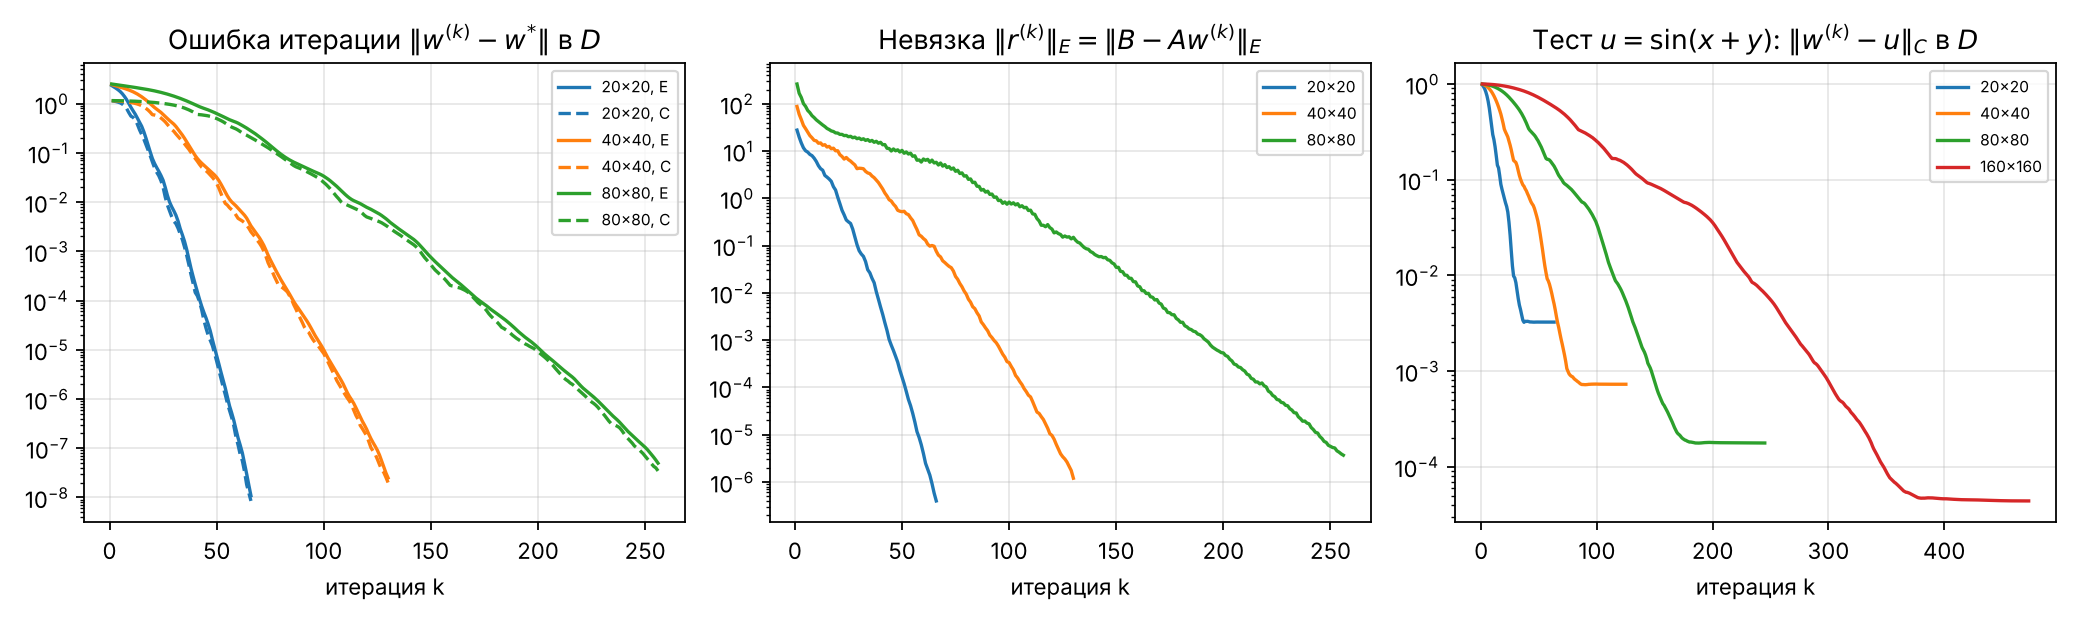
\includegraphics[width=\textwidth]{fig/conv_iter_err.png}
\caption{Ошибка по итерациям: относительно решения схемы (слева), невязка (в центре),
относительно точного решения в тестовой задаче (справа)}\label{fig:iter}
\end{figure}

\subsection*{Сходимость приближённого решения в области $D$}
Точное решение задачи неизвестно, поэтому погрешность оценивалась сравнением с решением
на подробной сетке $1280\times1280$ (эталон $w^{ref}$, $\delta=10^{-10}$). Нормы вычислялись
только по узлам, лежащим в области $D$ (фиктивная область не учитывалась):
$\|e\|_C=\max_{D}|w^h-w^{ref}|$, $\|e\|_E=\bigl(\sum_{D}h_1h_2(w^h-w^{ref})^2\bigr)^{1/2}$.

\begin{table}[H]\centering
\caption{Погрешность приближённого решения в области $D$}
\begin{tabular}{cccccc}\toprule
Сетка & $h$ & $\|e\|_C$ & порядок & $\|e\|_E$ & порядок \\\midrule
$20\times20$ & 0.2 & $2.02\cdot10^{-2}$ & -- & $1.01\cdot10^{-2}$ & -- \\
$40\times40$ & 0.1 & $3.85\cdot10^{-2}$ & -0.93 & $1.44\cdot10^{-2}$ & -0.51 \\
$80\times80$ & 0.05 & $2.93\cdot10^{-2}$ & 0.39 & $1.18\cdot10^{-2}$ & 0.28 \\
$160\times160$ & 0.025 & $1.83\cdot10^{-2}$ & 0.68 & $6.46\cdot10^{-3}$ & 0.87 \\
$320\times320$ & 0.0125 & $1.01\cdot10^{-2}$ & 0.85 & $3.05\cdot10^{-3}$ & 1.08 \\
$640\times640$ & 0.00625 & $5.08\cdot10^{-3}$ & 0.99 & $1.18\cdot10^{-3}$ & 1.37 \\
\bottomrule\end{tabular}
\end{table}
На грубых сетках ($h\ge0.1$) полукруг радиуса 1 покрывается всего 5--10 ячейками, и
погрешность ведёт себя немонотонно. Начиная с сетки $80\times80$ погрешность убывает
с первым порядком по $h$, что соответствует теоретической оценке метода фиктивных
областей ($\max_D|v-u|\le C\eps$ плюс $O(h)$ от аппроксимации границы ступенчатой
областью). Наибольшая погрешность сосредоточена у дуги $\gamma$ (рис.~\ref{fig:errmap}).
В фиктивной области решение отличается от $v_0$ не более чем на $1.3\cdot10^{-5}$
(сетка $80\times80$), то есть штрафной член работает правильно.

\begin{figure}[H]\centering
\begin{minipage}{0.49\textwidth}\centering
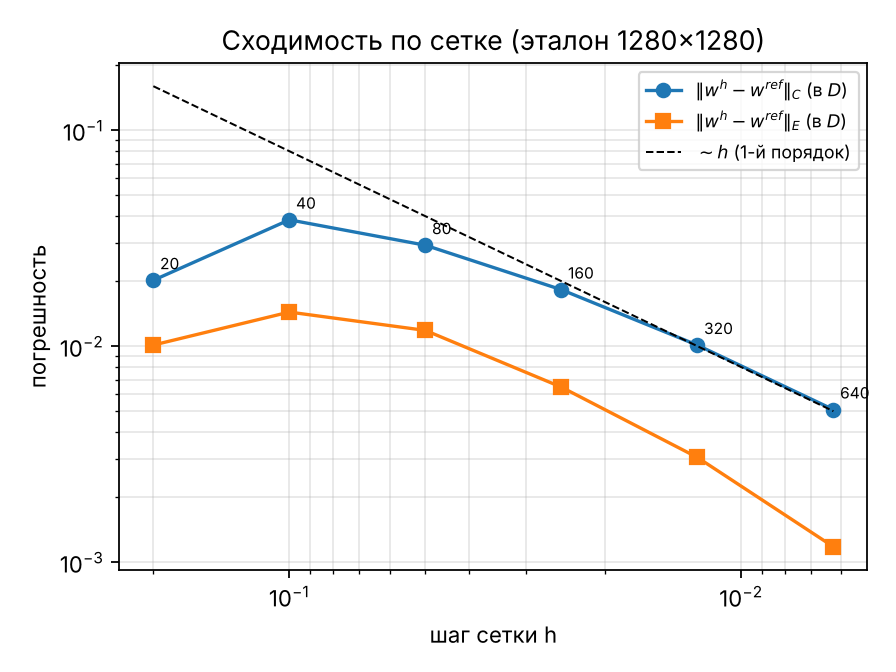
\includegraphics[width=\textwidth]{fig/conv_grid.png}
\caption{Погрешность в $D$ в зависимости от шага сетки}
\end{minipage}\hfill
\begin{minipage}{0.49\textwidth}\centering
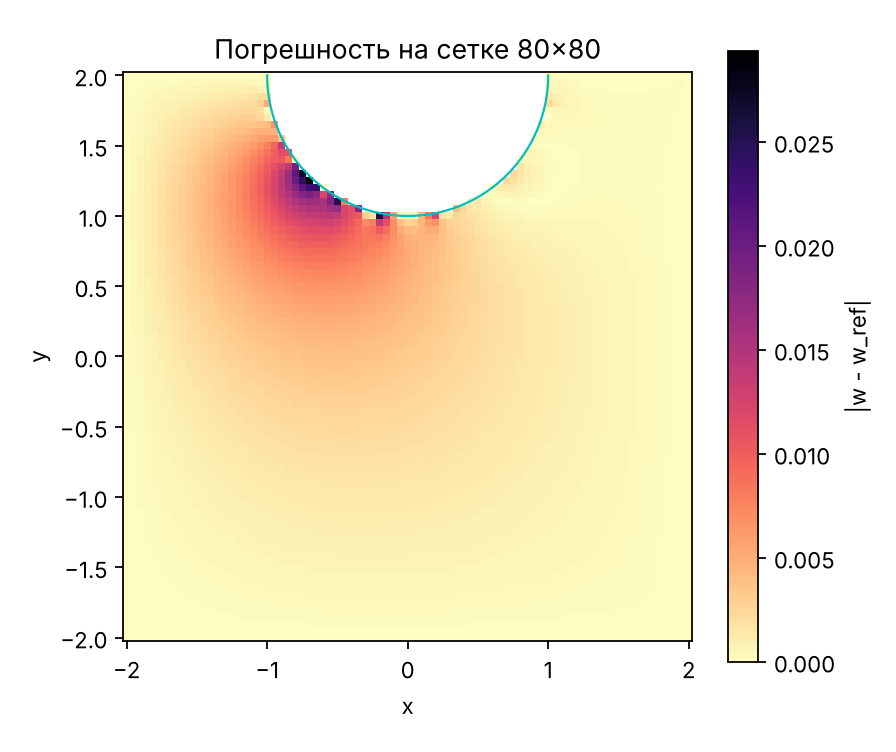
\includegraphics[width=\textwidth]{fig/error_map.png}
\caption{Распределение погрешности, сетка $80\times80$}\label{fig:errmap}
\end{minipage}
\end{figure}

\subsection*{Тест с точным решением}
Для проверки разностной схемы и решателя программа собирается с ключом \texttt{-DTEST\_EXACT}:
тогда $f(x,y)=2\sin(x+y)$, и точным решением задачи (1)--(2) является $u=\sin(x+y)$
(запуск \texttt{./seq M N delta - - exact} печатает ошибку в $D$). Поскольку продолжение
$v_0=\sin(x+y)$ совпадает с точным решением, погрешность метода фиктивных областей в этом
тесте исчезает, и проверяется порядок аппроксимации схемы и правильность решателя.

\begin{table}[H]\centering
\caption{Ошибка в области $D$ для тестовой задачи с точным решением $u=\sin(x+y)$}
\begin{tabular}{cccccc}\toprule
Сетка & $h$ & $\|w^h-u\|_C$ & порядок & $\|w^h-u\|_E$ & порядок \\\midrule
$20\times20$ & 0.2 & $3.25\cdot10^{-3}$ & -- & $5.78\cdot10^{-3}$ & -- \\
$40\times40$ & 0.1 & $7.28\cdot10^{-4}$ & 2.16 & $1.18\cdot10^{-3}$ & 2.29 \\
$80\times80$ & 0.05 & $1.77\cdot10^{-4}$ & 2.04 & $2.88\cdot10^{-4}$ & 2.04 \\
$160\times160$ & 0.025 & $4.39\cdot10^{-5}$ & 2.01 & $7.17\cdot10^{-5}$ & 2.01 \\
$320\times320$ & 0.0125 & $1.10\cdot10^{-5}$ & 2.00 & $1.79\cdot10^{-5}$ & 2.00 \\
$640\times640$ & 0.00625 & $2.74\cdot10^{-6}$ & 2.00 & $4.48\cdot10^{-6}$ & 2.00 \\
\bottomrule\end{tabular}
\end{table}
Ошибка убывает со вторым порядком по $h$, как и должно быть для пятиточечной схемы.
В основной задаче порядок первый (табл.~выше): его ограничивает аппроксимация криволинейной
границы $\gamma$ методом фиктивных областей, а не схема или решатель.

\begin{figure}[H]\centering
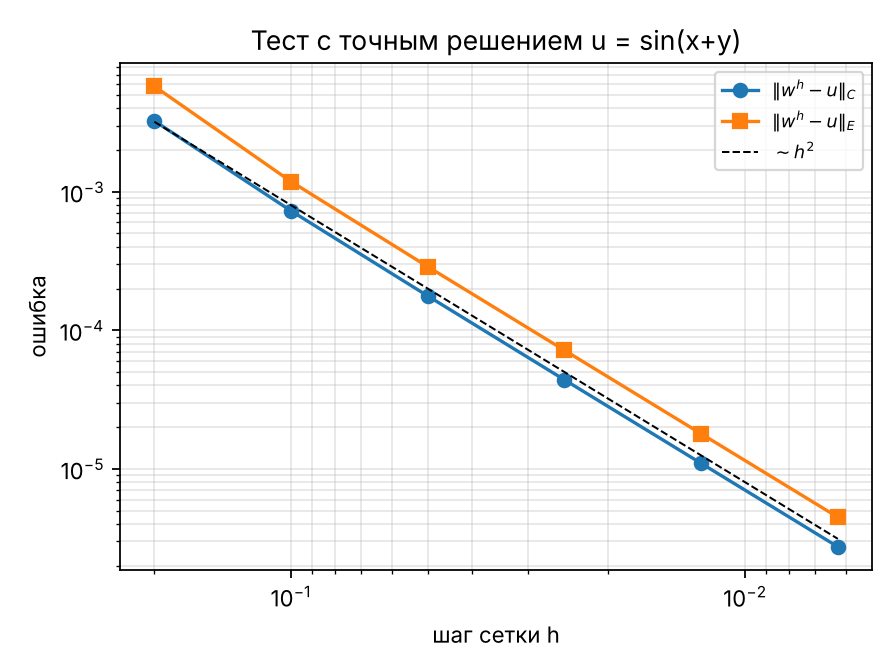
\includegraphics[width=0.55\textwidth]{fig/exact_grid.png}
\caption{Ошибка в тестовой задаче с точным решением}
\end{figure}

\section{OpenMP-программа}

Программа \texttt{omp.cpp} получена из последовательной добавлением директив
\texttt{\#pragma omp parallel for schedule(static)} к циклам по внешнему индексу $i$:
\begin{itemize}
\item формирование коэффициентов $Q_{ij}$, $B_{ij}$ и диагонали $D$;
\item применение оператора $A$;
\item векторные операции обновления $w$, $r$, $z$ и $p$;
\item скалярные произведения~--- с \texttt{reduction(+:s)}.
\end{itemize}
Обновления $w^{(k+1)}$, $r^{(k+1)}$ и $z^{(k+1)}$ объединены в один цикл, чтобы уменьшить
число проходов по памяти и число параллельных областей. Результат OpenMP-программы совпадает
с последовательным до $10^{-13}$ (различие только в порядке суммирования в редукциях)
при любом числе нитей; число итераций одинаковое.

\section{Разбиение на домены и MPI-программа}

\subsection*{Алгоритм двумерного разбиения}
Алгоритм вынесен в файл \texttt{partition.h} (общий для MPI- и гибридной версий).
Неизвестные~--- внутренние узлы $i=\overline{1,M-1}$, $j=\overline{1,N-1}$. Для числа процессов
$P$ перебираются все разложения $P=p_x\cdot p_y$. По каждому направлению узлы делятся на
$p_x$ (соответственно $p_y$) частей почти поровну: первые $n\bmod p$ частей получают
$\lfloor n/p\rfloor+1$ узлов, остальные~--- $\lfloor n/p\rfloor$. Поэтому размеры любых двух
доменов по каждой переменной различаются не более чем на единицу. Из разложений, для которых
отношение числа узлов по $x$ и $y$ в каждом домене лежит в $[1/2,2]$, выбирается то,
у которого отношение $\frac{(M-1)/p_x}{(N-1)/p_y}$ ближе всего к единице (минимум
$|\ln(\cdot)|$). Если допустимых разложений нет, берётся ближайшее к квадратным доменам.

\begin{table}[H]\centering
\caption{Разбиения, выбираемые программой}
\begin{tabular}{cccccc}\toprule
Сетка & $P$ & $p_x\times p_y$ & узлов по $x$ & узлов по $y$ & отношение $x/y$ \\\midrule
$80\times80$ & 2 & $1\times2$ & 79 & 39--40 & 1.98--2.03$^*$ \\
$80\times80$ & 4 & $2\times2$ & 39--40 & 39--40 & 0.97--1.03 \\
$400\times600$ & 2 & $1\times2$ & 399 & 299--300 & 1.33 \\
$400\times600$ & 4 & $2\times2$ & 199--200 & 299--300 & 0.66--0.67 \\
$400\times600$ & 8 & $2\times4$ & 199--200 & 149--150 & 1.33--1.34 \\
$400\times600$ & 16 & $4\times4$ & 99--100 & 149--150 & 0.66--0.67 \\
$800\times1200$ & 4 & $2\times2$ & 399--400 & 599--600 & 0.67 \\
$800\times1200$ & 8 & $2\times4$ & 399--400 & 299--300 & 1.33--1.34 \\
$800\times1200$ & 16 & $4\times4$ & 199--200 & 299--300 & 0.66--0.67 \\
$800\times1200$ & 32 & $4\times8$ & 199--200 & 149--150 & 1.33--1.34 \\\bottomrule
\end{tabular}

\smallskip
\small $^*$ Для квадратной сетки с 79 внутренними узлами и двух процессов условие $[1/2,2]$
нельзя выполнить точно: при любом разбиении один из доменов имеет 79 и 39 узлов.
Программа выбирает ближайшее допустимое разбиение.
\end{table}

\subsection*{Реализация}
Процессы объединяются в декартову топологию \texttt{MPI\_Cart\_create} размера
$p_x\times p_y$; соседи определяются \texttt{MPI\_Cart\_shift} (на границе $\Pi$ сосед
равен \texttt{MPI\_PROC\_NULL}). Каждый процесс хранит свой блок $n_x\times n_y$ с одним слоем
теневых узлов. Перед каждым применением оператора $A$ к $p^{(k)}$ выполняется обмен
граничными слоями с четырьмя соседями через \texttt{MPI\_Sendrecv}: строки по $x$
непрерывны в памяти, для столбцов используется производный тип \texttt{MPI\_Type\_vector}.
Теневые узлы на границе $\Gamma$ остаются нулевыми. Скалярные произведения вычисляются
локально и суммируются \texttt{MPI\_Allreduce}; на каждой итерации выполняются один обмен
и три глобальные редукции. Время~--- максимум \texttt{MPI\_Wtime} по процессам.
Для проверки решение собирается на процессе 0. Результаты MPI-программы при $P=1,2,4$ (и,
для проверки разбиения с остатками, при $P=6$ на сетке $37\times53$) совпадают с
последовательными до $10^{-12}$.

\section{Гибридная программа MPI+OpenMP}

Программа \texttt{hybrid.cpp}~--- это MPI-программа, в которой циклы по локальному блоку
распараллелены директивами OpenMP так же, как в \texttt{omp.cpp}. Обмены MPI и вызовы
\texttt{MPI\_Allreduce} выполняются главной нитью вне параллельных областей,
поэтому достаточно уровня поддержки потоков \texttt{MPI\_THREAD\_\allowbreak FUNNELED}.
Решение на сетке $80\times80$ при 1 и 2 процессах с 4 нитями совпадает с последовательным
до $10^{-12}$.

\section{Тестирование}
Набор тестов запускается командой \texttt{make test} (скрипт \texttt{tests/run\_tests.sh}) и
содержит 32 автоматические проверки; все они проходят.
\begin{enumerate}
\item \textbf{Площади и коэффициенты} (\texttt{tests/test\_geometry.cpp}, 14 проверок): площадь
всего полукруга и четверти круга по формуле совпадает с $\pi/2$ и $\pi/4$; сумма площадей
$\mathrm{mes}(\Pi_{ij}\cap\hat D)$ по всем ячейкам сеток разного размера равна $\pi/2$ с
точностью $10^{-12}$; для 200 случайных прямоугольников точная формула совпадает с численным
подсчётом; ячейки внутри $D$, в фиктивной области и на дуге получают правильные $Q_{ij}$ и $F_{ij}$.
\item \textbf{Разбиение на домены} (\texttt{tests/test\_partition.cpp}): для шести сеток и
$P=1,\dots,64$ (384 случая) проверено, что домены покрывают сетку без пропусков и пересечений,
а их размеры по каждой переменной отличаются не более чем на 1. Если отношение узлов
не попадает в $[1/2,2]$, тест перебором подтверждает, что допустимого разбиения нет.
Для всех конфигураций из таблиц 1--3 условие $[1/2,2]$ выполнено.
\item \textbf{Точное решение}: порядок сходимости на сетках $40,80,160$ лежит в $[1.8,\,2.3]$.
\item \textbf{Метод сопряжённых градиентов}: на сетках $20,40,80$ функционал $J$ не возрастает,
критерий остановки выполнен, число итераций не превосходит числа неизвестных; число итераций
совпадает с эталонным (66, 130, 256).
\item \textbf{Согласованность версий}: на сетках $80\times80$ и $37\times53$ (неравные размеры
доменов) OpenMP-версия на 1, 4, 16 нитях, MPI-версия на 1, 2, 4, 6 процессах и гибридная
на $1\times4$ и $2\times4$ дают то же число итераций, что и последовательная, а решения
отличаются не более чем на $10^{-12}$.
\end{enumerate}

\section{Результаты расчётов}

Число итераций определяется только сеткой и не зависит от числа нитей или процессов:
1499 для $400\times600$ и 2892 для $800\times1200$. Ускорение считается относительно
последовательной программы на Polus: $S=T_{\text{seq}}/T$, где $T_{\text{seq}}=11.72$~с
для $400\times600$ и $78.37$~с для $800\times1200$.

\begin{table}[H]\centering
\caption{Результаты расчётов на ПВС IBM Polus (OpenMP-код)}
\begin{tabular}{ccccc}\toprule
Число OpenMP-нитей & Сетка $M\times N$ & Число итераций & Время, с & Ускорение \\\midrule
\inputtable{tables/table1.tex}
\bottomrule\end{tabular}
\end{table}

\begin{table}[H]\centering
\caption{Результаты расчётов на ПВС IBM Polus (MPI-код)}
\begin{tabular}{ccccc}\toprule
Число процессов MPI & Сетка $M\times N$ & Число итераций & Время, с & Ускорение \\\midrule
\inputtable{tables/table2.tex}
\bottomrule\end{tabular}
\end{table}

\begin{table}[H]\centering
\caption{Результаты расчётов на ПВС IBM Polus (MPI+OpenMP-код)}
\begin{tabular}{cccccc}\toprule
Процессы MPI & Нитей в процессе & Сетка $M\times N$ & Итераций & Время, с & Ускорение \\\midrule
\inputtable{tables/table3.tex}
\bottomrule\end{tabular}
\end{table}

\paragraph{Проверка на сетке $80\times80$ (пп.~2, 5, 7 задания).}
Все параллельные версии дают то же число итераций и то же решение, что и последовательная
программа (разница до $10^{-12}$). На такой маленькой сетке расчёт занимает около 50~мс, и
накладные расходы на синхронизацию нитей и обмены сопоставимы с вычислениями.

\begin{table}[H]\centering
\caption{Сетка $80\times80$, IBM Polus (256 итераций во всех запусках)}
\begin{tabular}{lcc}\toprule
Программа & Время, с & Ускорение \\\midrule
Последовательная & 0.0452 & 1.00 \\
OpenMP, 1 нить & 0.0746 & 0.61 \\
OpenMP, 4 нити & 0.0242 & 1.87 \\
OpenMP, 16 нитей & 0.0287 & 1.57 \\
MPI, 1 процесс & 0.0361 & 1.25 \\
MPI, 2 процесса & 0.0216 & 2.09 \\
MPI, 4 процесса & 0.0134 & 3.37 \\
MPI+OpenMP, $1\times4$ & 0.0284 & 1.59 \\
MPI+OpenMP, $2\times4$ & 0.0300 & 1.51 \\
\bottomrule
\end{tabular}
\end{table}

\paragraph{Условия запуска.} Расчёты выполнены на ПВС IBM Polus (узлы с двумя процессорами
IBM Power8, по 10 ядер, 8 SMT-нитей на ядро). Компилятор GCC с ключом \texttt{-O1}, библиотека
IBM Spectrum MPI. Задания ставились в очередь LSF (\texttt{bsub}) с привязкой к ядрам
(\texttt{affinity[core(N)]}) и размещением не более 20 ядер на узел
(\texttt{span[ptile=\dots]}). Каждое задание занимало узел эксклюзивно (\texttt{bsub -x}) и запускалось три раза; в таблицы
внесено наименьшее время.

\paragraph{Анализ.}
Времена трёх повторных запусков каждого задания различаются менее чем на 1\%, поэтому
приведённые значения воспроизводимы.
\begin{itemize}
\item MPI-версия масштабируется лучше всего: на сетке $800\times1200$ при 32 процессах ускорение
составило 33.6, на сетке $400\times600$ при 16 процессах~--- 19.0. Ускорение больше числа
процессов (сверхлинейное) объясняется кэшем: восемь сеточных массивов задачи $800\times1200$
занимают около 77~МБ, а при 32 процессах на один процесс приходится около 2.4~МБ, что
помещается в кэш L2+L3 ядра Power8 (512~КБ + 8~МБ). Обращения к оперативной памяти почти
исчезают, и каждая итерация выполняется быстрее, чем в последовательной программе.
\item OpenMP-версия даёт ускорение около 4.2 на 8--16 нитях (сетка $400\times600$) и 7.2 на
32 нитях (сетка $800\times1200$). Метод сопряжённых градиентов состоит из простых операций
над векторами (шаблон <<крест>>, скалярные произведения), поэтому на одном узле его
производительность ограничена пропускной способностью памяти, а не числом ядер.
\item Гибридная версия на 4 процессах по 8 нитей (сетка $800\times1200$) даёт ускорение 30.3,
на 2 процессах по 8 нитей (сетка $400\times600$)~--- 16.0, что сравнимо с MPI-версией на том
же числе ядер.
\item Ускорение MPI-версии растёт немонотонно: на сетке $400\times600$ при 4 процессах (1.77)
оно меньше, чем при 2 (2.55), а на сетке $800\times1200$ при 16 процессах (7.9)~--- меньше,
чем при 8 (8.8). Эффект воспроизводится во всех повторах и при эксклюзивном доступе к узлу,
то есть не связан с посторонней нагрузкой; гибридная версия с одной нитью на процесс
($4\times1$) показывает то же время, что и MPI на 4 процессах. Наиболее вероятная причина~---
размещение процессов по ядрам и процессорам узла, которое задаётся планировщиком LSF
(\texttt{affinity[core(1)]}): при неудачной раскладке процессы делят кэш и контроллер памяти
одного процессора.
\end{itemize}

\section{Рисунки}

\begin{figure}[H]\centering
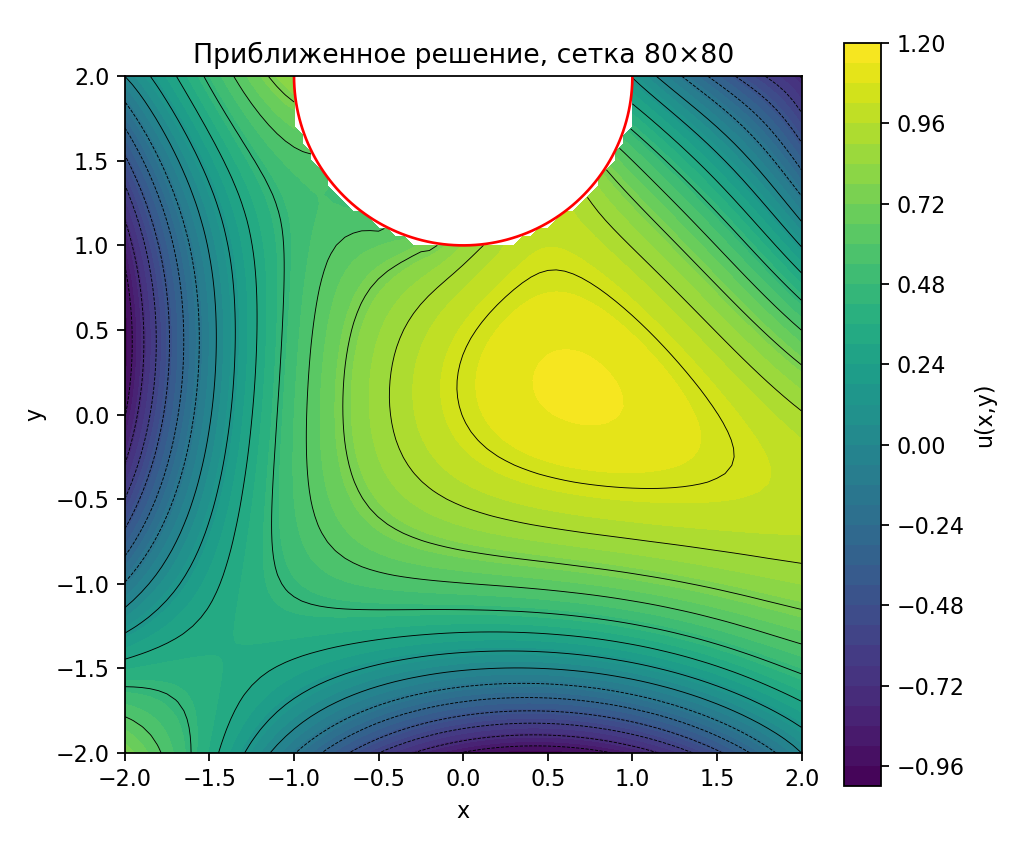
\includegraphics[width=0.62\textwidth]{fig/solution_map.png}
\caption{Приближенное решение на сетке $800\times1200$ (линии уровня, красным~--- дуга $\gamma$)}
\end{figure}
\begin{figure}[H]\centering
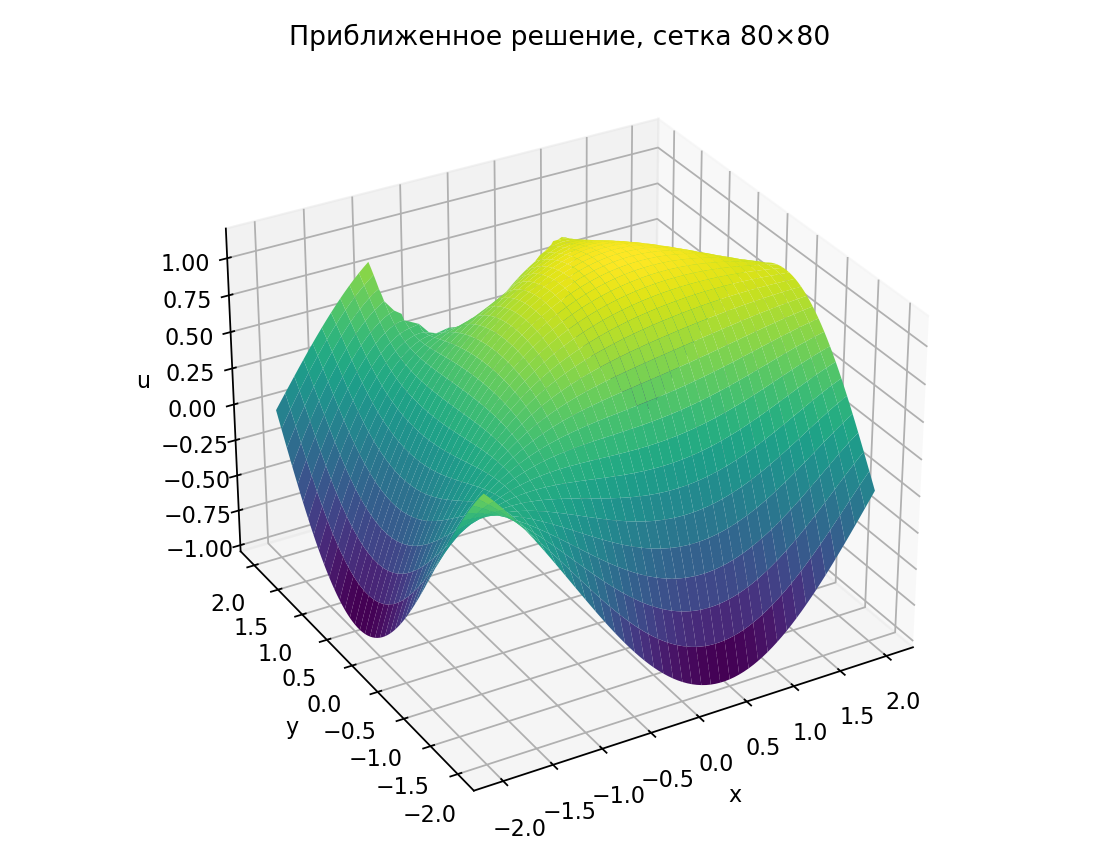
\includegraphics[width=0.68\textwidth]{fig/solution_3d.png}
\caption{Приближенное решение на сетке $800\times1200$ (фиктивная область исключена)}
\end{figure}

\IfFileExists{fig/speedup_omp.png}{
\begin{figure}[H]\centering
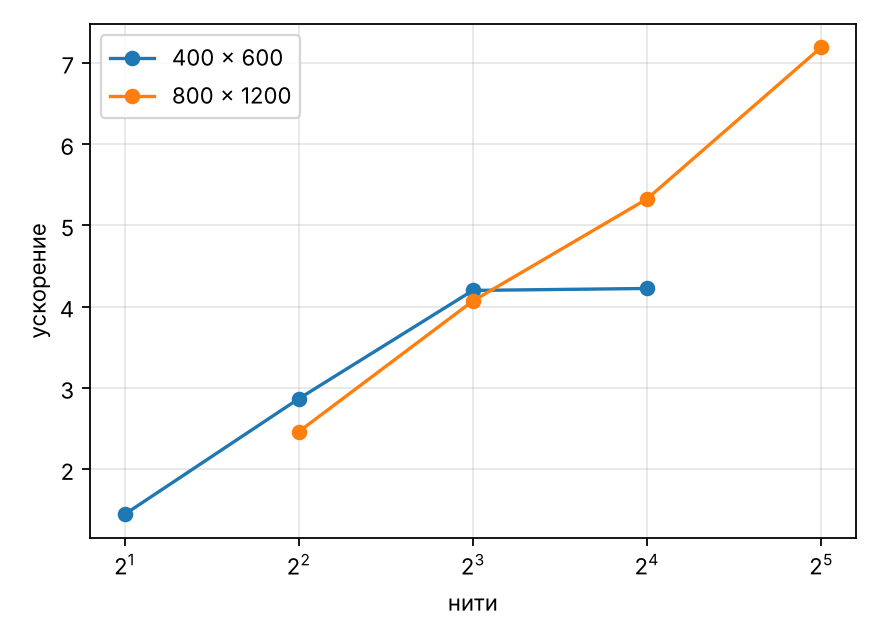
\includegraphics[width=0.6\textwidth]{fig/speedup_omp.png}
\caption{Ускорение OpenMP-программы на IBM Polus}\end{figure}}{}
\IfFileExists{fig/speedup_mpi.png}{
\begin{figure}[H]\centering
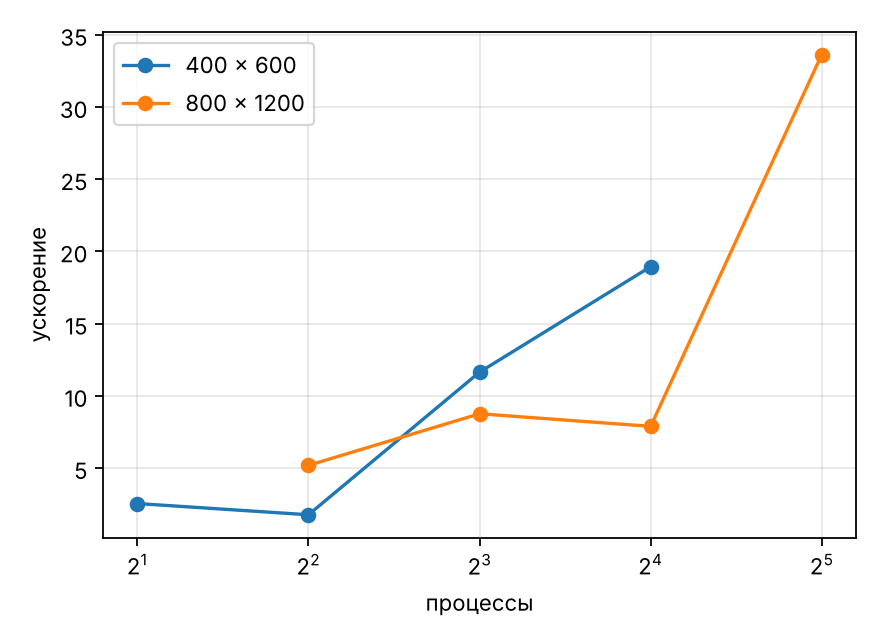
\includegraphics[width=0.6\textwidth]{fig/speedup_mpi.png}
\caption{Ускорение MPI-программы на IBM Polus}\end{figure}}{}
\IfFileExists{fig/speedup_hybrid.png}{
\begin{figure}[H]\centering
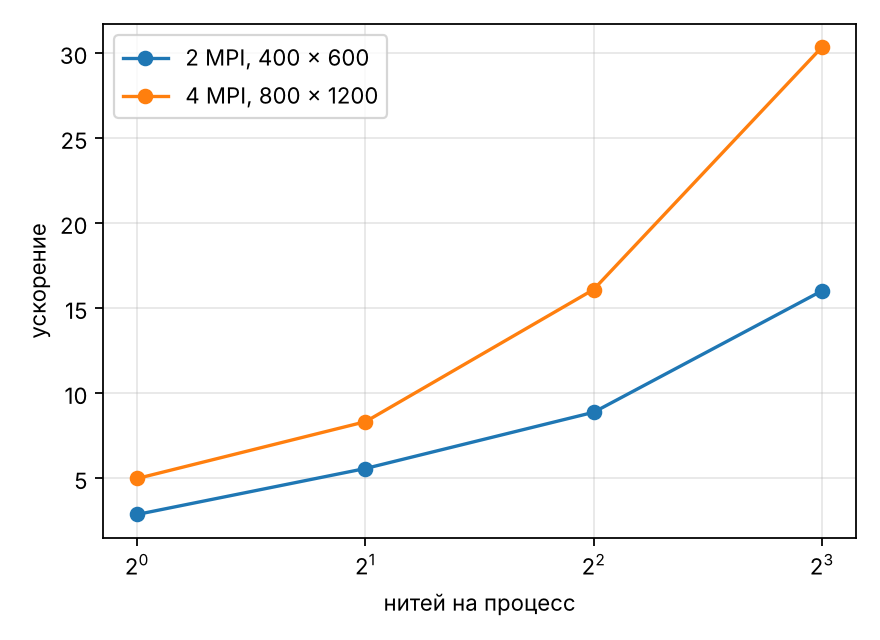
\includegraphics[width=0.6\textwidth]{fig/speedup_hybrid.png}
\caption{Ускорение гибридной программы на IBM Polus}\end{figure}}{}



\section{Выводы}
\begin{itemize}
\item Задача Дирихле в области <<квадрат без полукруга>> сведена методом фиктивных областей к
задаче в квадрате $\Pi=(-2,2)^2$; площади пересечения ячеек с областью вычисляются точно.
\item Метод сопряжённых градиентов с диагональным предобуславливанием сходится за
$O(\max(M,N))$ итераций, несмотря на большой штраф $1/\eps^2=h^{-4}$.
\item Реализованы OpenMP-, MPI- и гибридная версии; все они дают решение, совпадающее
с последовательным с точностью до ошибок округления, и одинаковое число итераций.
\item Реализовано двумерное разбиение на домены с почти квадратными блоками,
что минимизирует объём обменов.
\item Приближённое решение сходится в области $D$ с первым порядком по $h$; в тесте с точным
решением схема показывает второй порядок. Итерационная ошибка при $\delta=10^{-8}$ на
4 порядка меньше погрешности сетки.
\item Корректность кода подтверждается набором из 32 автоматических тестов (\texttt{make test}).
\end{itemize}

\section*{Приложение. Сборка и запуск}
Исходный код, тесты, скрипты и результаты расчётов: \url{GITHUB_URL}
\begin{verbatim}
make                                     # seq, omp, mpi, hybrid (флаги -O1)
make test                                # 32 автоматических теста
./seq 80 80 1e-8 sol.txt                 # M N delta [файл решения]
./seq 80 80 1e-8 - tr.txt ref.txt        # журнал итераций и ошибка относительно ref.txt
OMP_NUM_THREADS=4 ./omp 400 600
mpirun -np 4 ./mpi 400 600
OMP_NUM_THREADS=4 mpirun -np 2 ./hybrid 400 600
bash scripts/polus_all.sh                # все расчеты на Polus -> results/polus
python3 scripts/collect.py               # таблицы 1-3 и графики ускорения
python3 scripts/plot_convergence.py      # графики сходимости и ошибки
\end{verbatim}

\begin{thebibliography}{9}
\bibitem{} А.Н. Тихонов, А.А. Самарский. Уравнения математической физики. М.: Наука, 1977.
\bibitem{} Г.И. Марчук. Методы вычислительной математики. М.: Наука, 1989.
\bibitem{} П.Н. Вабищевич. Метод фиктивных областей в задачах математической физики. 2017.
\bibitem{} А.А. Самарский. Теория разностных схем. М.: Наука, 1989.
\bibitem{} А.А. Самарский, А.В. Гулин. Численные методы. М.: Наука, 1989.
\bibitem{} IBM Polus~--- \url{http://hpc.cmc.msu.ru}
\end{thebibliography}

\end{document}
